\section{立体几何的几何法证明}

\section{线线平行 (Line-Line Parallel)}

% --- 判定定理 1 ---
\begin{theorem}[平行公理的推论]
    平行于同一条直线的两条直线互相平行。
    \begin{equation*}
        \left.
        \begin{array}{l}
            l \parallel n \\
            m \parallel n
        \end{array}
        \right\} \implies l \parallel m
    \end{equation*}
\end{theorem}

\begin{center}
    \begin{tikzpicture}[scale=1.2]
        % 定义坐标
        \coordinate (A) at (0,0,0);
        \coordinate (B) at (4,0,0);
        \coordinate (C) at (0,1,1);
        \coordinate (D) at (4,1,1);
        \coordinate (E) at (0,2,-0.5);
        \coordinate (F) at (4,2,-0.5);

        % 绘制直线
        \draw[thick] (A) -- (B) node[right]{$l$};
        \draw[thick] (C) -- (D) node[right]{$m$};
        \draw[thick] (E) -- (F) node[right]{$n$};
    \end{tikzpicture}
\end{center}


% --- 性质定理 1 ---
\begin{theorem}
    如果两条平行线中的一条垂直于一个平面，那么另一条也垂直于该平面。
    \begin{equation*}
        \left.
        \begin{array}{l}
            l \parallel m \\
            l \perp \alpha
        \end{array}
        \right\} \implies m \perp \alpha
    \end{equation*}
\end{theorem}

\begin{center}
    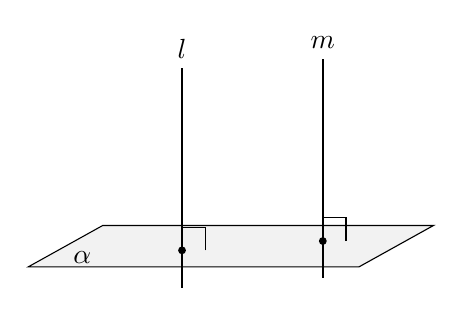
\begin{tikzpicture}[
            scale=1.05,
            x={(1cm,0cm)},
            y={(0.45cm,0.25cm)},
            z={(0cm,1cm)},
            point/.style={circle, fill=black, inner sep=1pt}
        ]
        \coordinate (A) at (0,0,0);
        \coordinate (B) at (4,0,0);
        \coordinate (C) at (4,2,0);
        \coordinate (D) at (0,2,0);
        \coordinate (O1) at (1.5,0.8,0);
        \coordinate (O2) at (3,1.25,0);

        \draw[fill=gray!10] (A) -- (B) -- (C) -- (D) -- cycle;
        \node at (0.45,0.45,0) {$\alpha$};
        \draw[thick] (O1) -- ++(0,0,2.2) node[above] {$l$};
        \draw[thick] (O1) -- ++(0,0,-0.45);
        \draw[thick] (O2) -- ++(0,0,2.2) node[above] {$m$};
        \draw[thick] (O2) -- ++(0,0,-0.45);
        \node[point] at (O1) {};
        \node[point] at (O2) {};
        \draw (O1) ++(0.28,0,0) -- ++(0,0,0.28) -- ++(-0.28,0,0);
        \draw (O2) ++(0.28,0,0) -- ++(0,0,0.28) -- ++(-0.28,0,0);
    \end{tikzpicture}
\end{center}

\newpage

\section{线面平行 (Line-Plane Parallel)}

% --- 判定定理 2 ---
\begin{theorem}
    如果平面外一条直线与此平面内的一条直线平行，那么该直线与此平面平行。
    \begin{equation*}
        \left.
        \begin{array}{l}
            l \not\subset \alpha, m \subset \alpha \\
            l \parallel m
        \end{array}
        \right\} \implies l \parallel \alpha
    \end{equation*}
\end{theorem}

\begin{center}
    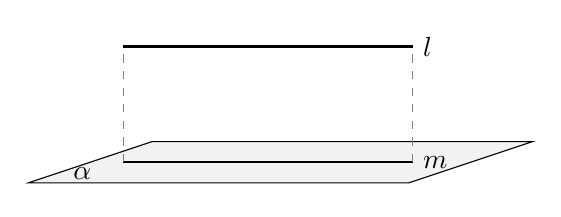
\begin{tikzpicture}[
            scale=1.05,
            x={(1cm,0cm)},
            y={(0.45cm,0.25cm)},
            z={(0cm,1cm)}
        ]
        \coordinate (A) at (0,0,0);
        \coordinate (B) at (4.6,0,0);
        \coordinate (C) at (5.2,2,0);
        \coordinate (D) at (0.6,2,0);

        \draw[fill=gray!10] (A) -- (B) -- (C) -- (D) -- cycle;
        \node at (0.45,0.45,0) {$\alpha$};
        \draw[thick] (0.7,1,0) -- (4.2,1,0) node[right] {$m$};
        \draw[thick] (0.7,1,1.4) -- (4.2,1,1.4) node[right] {$l$};
        \draw[dashed, gray] (0.7,1,0) -- (0.7,1,1.4);
        \draw[dashed, gray] (4.2,1,0) -- (4.2,1,1.4);
    \end{tikzpicture}
\end{center}

% --- 性质定理 2 ---
\begin{theorem}
    如果一条直线与一个平面平行，则过这条直线的任一平面与此平面的交线与该直线平行。
    \begin{equation*}
        \left.
        \begin{array}{l}
            l \parallel \alpha, l \subset \beta \\
            \alpha \cap \beta = m
        \end{array}
        \right\} \implies l \parallel m
    \end{equation*}
\end{theorem}
\begin{center}
    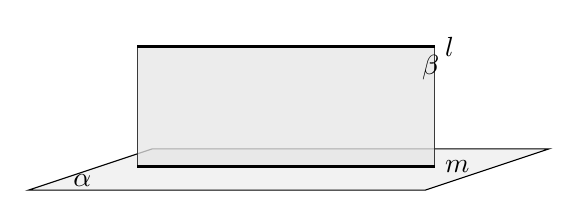
\begin{tikzpicture}[
            scale=1.05,
            x={(1cm,0cm)},
            y={(0.45cm,0.25cm)},
            z={(0cm,1cm)}
        ]
        \coordinate (A) at (0,0,0);
        \coordinate (B) at (4.8,0,0);
        \coordinate (C) at (5.4,2,0);
        \coordinate (D) at (0.6,2,0);
        \coordinate (M1) at (0.8,1.15,0);
        \coordinate (M2) at (4.4,1.15,0);
        \coordinate (L1) at (0.8,1.15,1.45);
        \coordinate (L2) at (4.4,1.15,1.45);

        \draw[fill=gray!10] (A) -- (B) -- (C) -- (D) -- cycle;
        \draw[fill=gray!20, opacity=0.75] (M1) -- (M2) -- (L2) -- (L1) -- cycle;
        \node at (0.45,0.45,0) {$\alpha$};
        \node at (4.35,1.15,1.2) {$\beta$};
        \draw[thick] (L1) -- (L2) node[right] {$l$};
        \draw[thick] (M1) -- (M2) node[right] {$m$};
    \end{tikzpicture}
\end{center}

\newpage

\section{线面垂直 (Line-Plane Perpendicular)}

% --- 判定定理 3 ---
\begin{theorem}
    如果一条直线与一个平面内的两条相交直线都垂直，那么该直线与此平面垂直。
    \begin{equation*}
        \left.
        \begin{array}{l}
            m \subset \alpha, n \subset \alpha, m \cap n = O \\
            l \perp m, l \perp n
        \end{array}
        \right\} \implies l \perp \alpha
    \end{equation*}
\end{theorem}
\begin{center}
    \begin{tikzpicture}[
            scale=1.05,
            x={(1cm,0cm)},
            y={(0.45cm,0.25cm)},
            z={(0cm,1cm)},
            point/.style={circle, fill=black, inner sep=1pt}
        ]
        \coordinate (A) at (0,0,0);
        \coordinate (B) at (4.2,0,0);
        \coordinate (C) at (4.8,2,0);
        \coordinate (D) at (0.6,2,0);
        \coordinate (O) at (2.35,1,0);

        \draw[fill=gray!10] (A) -- (B) -- (C) -- (D) -- cycle;
        \node at (0.45,0.45,0) {$\alpha$};
        \draw[thick] ($(O)+(-1.55,0,0)$) -- ($(O)+(1.7,0,0)$) node[right] {$m$};
        \draw[thick] ($(O)+(0,-0.95,0)$) -- ($(O)+(0,1.05,0)$) node[above right] {$n$};
        \draw[thick] (O) -- ++(0,0,2.1) node[above] {$l$};
        \draw[thick] (O) -- ++(0,0,-0.45);
        \node[point, label=below right:$O$] at (O) {};
        \draw (O) ++(0.28,0,0) -- ++(0,0,0.28) -- ++(-0.28,0,0);
        \draw (O) ++(0,0.28,0) -- ++(0,0,0.28) -- ++(0,-0.28,0);
    \end{tikzpicture}
\end{center}

% --- 性质定理 3 ---
\begin{theorem}
    垂直于同一个平面的两条直线平行。
    \begin{equation*}
        \left.
        \begin{array}{l}
            l \perp \alpha \\
            m \perp \alpha
        \end{array}
        \right\} \implies l \parallel m
    \end{equation*}
\end{theorem}
\begin{center}
    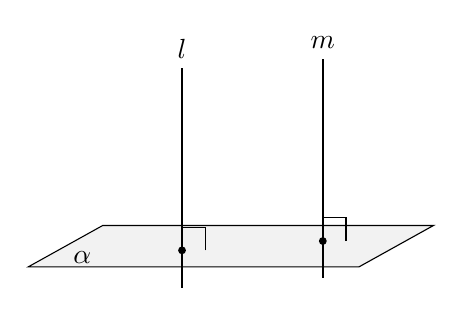
\begin{tikzpicture}[
            scale=1.05,
            x={(1cm,0cm)},
            y={(0.45cm,0.25cm)},
            z={(0cm,1cm)},
            point/.style={circle, fill=black, inner sep=1pt}
        ]
        \coordinate (A) at (0,0,0);
        \coordinate (B) at (4,0,0);
        \coordinate (C) at (4,2,0);
        \coordinate (D) at (0,2,0);
        \coordinate (O1) at (1.5,0.8,0);
        \coordinate (O2) at (3,1.25,0);

        \draw[fill=gray!10] (A) -- (B) -- (C) -- (D) -- cycle;
        \node at (0.45,0.45,0) {$\alpha$};
        \draw[thick] (O1) -- ++(0,0,2.2) node[above] {$l$};
        \draw[thick] (O1) -- ++(0,0,-0.45);
        \draw[thick] (O2) -- ++(0,0,2.2) node[above] {$m$};
        \draw[thick] (O2) -- ++(0,0,-0.45);
        \node[point] at (O1) {};
        \node[point] at (O2) {};
        \draw (O1) ++(0.28,0,0) -- ++(0,0,0.28) -- ++(-0.28,0,0);
        \draw (O2) ++(0.28,0,0) -- ++(0,0,0.28) -- ++(-0.28,0,0);
    \end{tikzpicture}
\end{center}

\newpage

\section{面面垂直 (Plane-Plane Perpendicular)}

% --- 判定定理 4 ---
\begin{theorem}
    如果一个平面经过另一个平面的一条垂线，那么这两个平面互相垂直。
    \begin{equation*}
        \left.
        \begin{array}{l}
            l \subset \beta \\
            l \perp \alpha
        \end{array}
        \right\} \implies \alpha \perp \beta
    \end{equation*}
\end{theorem}
\begin{center}
    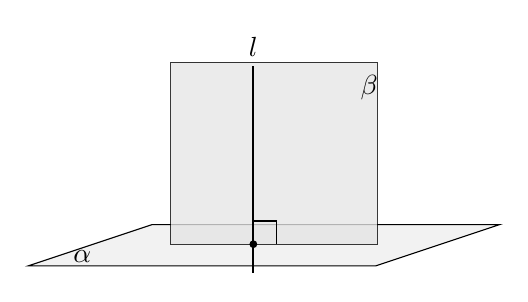
\begin{tikzpicture}[
            scale=1.05,
            x={(1cm,0cm)},
            y={(0.45cm,0.25cm)},
            z={(0cm,1cm)},
            point/.style={circle, fill=black, inner sep=1pt}
        ]
        \coordinate (A) at (0,0,0);
        \coordinate (B) at (4.2,0,0);
        \coordinate (C) at (4.8,2,0);
        \coordinate (D) at (0.6,2,0);
        \coordinate (P1) at (1.25,1.05,0);
        \coordinate (P2) at (3.75,1.05,0);
        \coordinate (Q1) at (1.25,1.05,2.2);
        \coordinate (Q2) at (3.75,1.05,2.2);
        \coordinate (O) at (2.25,1.05,0);

        \draw[fill=gray!10] (A) -- (B) -- (C) -- (D) -- cycle;
        \draw[fill=gray!20, opacity=0.78] (P1) -- (P2) -- (Q2) -- (Q1) -- cycle;
        \node at (0.45,0.45,0) {$\alpha$};
        \node at (3.65,1.05,1.9) {$\beta$};
        \draw[thick] (O) -- ++(0,0,2.15) node[above] {$l$};
        \draw[thick] (O) -- ++(0,0,-0.35);
        \node[point] at (O) {};
        \draw (O) ++(0.28,0,0) -- ++(0,0,0.28) -- ++(-0.28,0,0);
    \end{tikzpicture}
\end{center}

% --- 性质定理 4 ---
\begin{theorem}
    如果两个平面互相垂直，那么在一个平面内垂直于它们交线的直线垂直于另一个平面。
    \begin{equation*}
        \left.
        \begin{array}{l}
            \alpha \perp \beta, \alpha \cap \beta = l \\
            m \subset \alpha, m \perp l
        \end{array}
        \right\} \implies m \perp \beta
    \end{equation*}
\end{theorem}
\begin{center}
    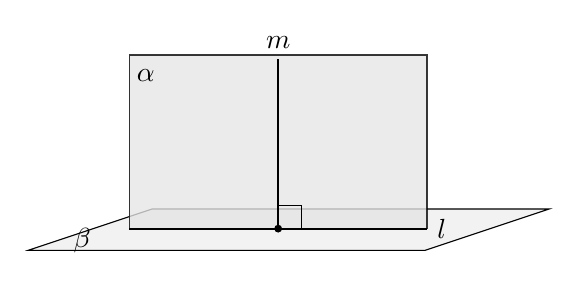
\begin{tikzpicture}[
            scale=1.05,
            x={(1cm,0cm)},
            y={(0.45cm,0.25cm)},
            z={(0cm,1cm)},
            point/.style={circle, fill=black, inner sep=1pt}
        ]
        \coordinate (A) at (0,0,0);
        \coordinate (B) at (4.8,0,0);
        \coordinate (C) at (5.4,2,0);
        \coordinate (D) at (0.6,2,0);
        \coordinate (L1) at (0.75,1.05,0);
        \coordinate (L2) at (4.35,1.05,0);
        \coordinate (U1) at (0.75,1.05,2.1);
        \coordinate (U2) at (4.35,1.05,2.1);
        \coordinate (O) at (2.55,1.05,0);

        \draw[fill=gray!10] (A) -- (B) -- (C) -- (D) -- cycle;
        \draw[fill=gray!20, opacity=0.78] (L1) -- (L2) -- (U2) -- (U1) -- cycle;
        \node at (0.45,0.45,0) {$\beta$};
        \node at (0.95,1.05,1.85) {$\alpha$};
        \draw[thick] (L1) -- (L2) node[right] {$l$};
        \draw[thick] (O) -- ++(0,0,2.05) node[above] {$m$};
        \node[point] at (O) {};
        \draw (O) ++(0.28,0,0) -- ++(0,0,0.28) -- ++(-0.28,0,0);
    \end{tikzpicture}
\end{center}

\subsection{证明线面平行}

\begin{example}
    如图，$A B C D$ 是边长为3的正方形，$D E \perp$ 平面 $A B C D, ~ A F / / D E$ 且 $D E=2 A F=4$ ．
    \begin{enumerate}
        \item 求证：$B F / /$ 平面 $D E C$ ；
        \item 求平面 $B E C$ 与平面 $B E F$ 夹角的余弦值；
        \item 求点 $D$ 到平面 $B E F$ 的距离.
    \end{enumerate}
\end{example}

\begin{figure} [H]
    \centering
    \resizebox{0.2\textwidth}{!}{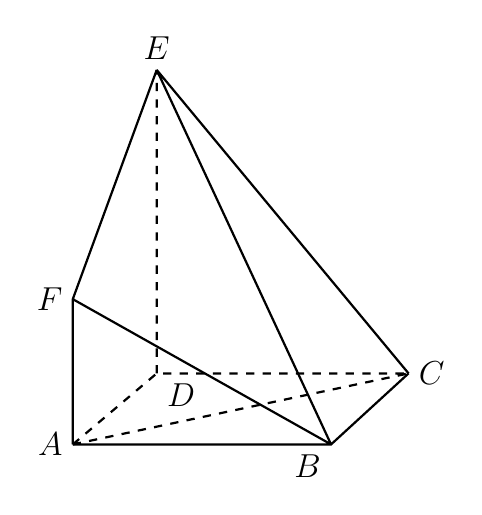
\begin{tikzpicture}[scale=.82,font=\large,thick]
\coordinate(A)at(-2.2,0);\coordinate(B)at(1.8,0);\coordinate(C)at(3,1.1);\coordinate(D)at(-.9,1.1);
\coordinate(E)at(-.9,5.8);\coordinate(F)at(-2.2,2.25);
\draw(A)--(B)--(C) (A)--(F)--(E) (F)--(B) (E)--(B) (E)--(C);
\draw[dashed](A)--(D)--(C) (D)--(E) (A)--(C);
\foreach\p/\pos in{E/above,A/left,B/below left,C/right,D/below right,F/left}{\node[\pos]at(\p){$\p$};}
\end{tikzpicture}
}
\end{figure}

\begin{example}
    如图，四棱锥 $P-A B C D$ 中，$P D \perp D A, P D \perp D C$ ，在底面 $A B C D$ 中，$A B \| D C, ~ A B \perp A D$ ，且 $2 A B=C D=6$ ， $A D=P D=4, ~ E$ 为 $P C$ 的中点．
    \begin{enumerate}
        \item 求证：$B E / /$ 平面 $A D P$ ；
        \item 求异面直线 $P A$ 与 $B C$ 所成的角的余弦值．
    \end{enumerate}
\end{example}

\begin{figure} [H]
    \centering
    \resizebox{0.2\textwidth}{!}{\begin{tikzpicture}[scale=.7,font=\large,thick]
\coordinate(P)at(0,5.7);\coordinate(A)at(-1.9,0);\coordinate(B)at(1.4,0);\coordinate(C)at(6.4,1.5);\coordinate(D)at(0,1.5);
\coordinate(E)at($(P)!.52!(C)$);
\draw(P)--(A)--(B)--(C)--(P) (P)--(B) (B)--(E);\draw[dashed](P)--(D)--(A) (D)--(C);
\foreach\p/\pos in{P/above,A/below left,B/below,C/right,D/left,E/above}{\node[\pos]at(\p){$\p$};}
\end{tikzpicture}
}
\end{figure}

\subsection{证明线线垂直}

\begin{theorem}[线面垂直的性质]

\end{theorem}

\begin{example}
    如图，四棱雉 $S-A B C D$ 的底面是边长为 2 的正方形，每条侧棱的长都是底面边长的 $\sqrt{2}$ 倍，$P$ 为侧棱 $S D$ 上的点，且 $S B / /$ 平面 $P A C$ ．
    \begin{enumerate}
        \item 求证：$A C \perp S D$ ．

        \item 求直线 $S B$ 到平面 $P A C$ 的距离．

        \item 请判断在平面 $P A C$ 上是否存在一点 $E$ ，使得 $\triangle E S B$ 是以 $S B$ 为底边，$\frac{2 \pi}{3}$ 为顶角的等腰三角形．若存在，请求出点 $E$ 的轨迹；若不存在，请说明理由．
    \end{enumerate}
\end{example}

\begin{figure} [H]
    \centering
    \resizebox{0.2\textwidth}{!}{\begin{tikzpicture}[scale=.72,font=\large,thick]
\coordinate(S)at(.96,6.3);\coordinate(A)at(-.6,1.7);\coordinate(B)at(-3,0);\coordinate(C)at(2.4,0);\coordinate(D)at(4.8,1.7);
\coordinate(P)at($(S)!.48!(D)$);
\draw(S)--(B)--(C)--(D)--(S) (S)--(C) (P)--(C);\draw[dashed](S)--(A)--(B) (A)--(C) (A)--(D) (B)--(P);
\foreach\p/\pos in{S/above,A/left,B/below left,C/below,D/right,P/right}{\node[\pos]at(\p){$\p$};}
\end{tikzpicture}
}
\end{figure}

\section{证明线面垂直}

\begin{example}
    底面为菱形的四棱雉 $P-A B C D$ 中，$A C$ 与 $B D$ 交于点 $O$ ，平面 $P B D \perp$ 平面 $A B C D$ ，平面 $P A C \perp$ 平面 $A B C D$ ．
    \begin{enumerate}
        \item 证明：$P O \perp$ 平面 $A B C D$ ；

        \item 若 $O A=2 O D=2$ ，直线 $D C$ 与平面 $P B C$ 所成角的正弦值为 $\frac{4 \sqrt{5}}{15}$ ，求平面 $P A C$ 与平面 $P B C$ 夹角的余弦值．
    \end{enumerate}
\end{example}

\begin{figure} [H]
    \centering
    \resizebox{0.2\textwidth}{!}{\begin{tikzpicture}[scale=.66,font=\large,thick]
\coordinate(P)at(.9,7.2);\coordinate(A)at(-3.6,0);\coordinate(B)at(2.4,0);\coordinate(D)at(-.55,1.8);\coordinate(C)at(5.45,1.8);
\coordinate(O)at($(A)!.5!(C)$);
\draw(P)--(A)--(B)--(C)--(P) (P)--(B);\draw[dashed](P)--(D)--(A) (D)--(C) (A)--(C) (D)--(B) (P)--(O);
\foreach\p/\pos in{P/above,A/below left,B/below,C/right,D/left,O/below}{\node[\pos]at(\p){$\p$};}
\end{tikzpicture}
}
\end{figure}
